% % % % % % % % % % % % % % % % % % % % % % % % % % % % % % % % % % % % % % % %
% IEEE Style - Double columns, 11pt font, letterpaper
\documentclass[journal, twocolumn, final,11pt,letterpaper]{IEEEtran}	

% Include Latex Packages
\usepackage{etex}	% This package enables the use of many packages

% % Page styles
\usepackage{setspace}	% line spacing package
\doublespacing			% use double spacing
%\linespread{1.6}		% Use linespread to fine tune line spacing, not recommended


% % Figures
\usepackage{float}		% improves interface for floating objects
\usepackage{subfig}		% enables subfloat
\usepackage{graphicx}	% more image type support
\usepackage{circuitikz}
\usepackage{epstopdf}	% automatically convert included eps files to pdf
\usepackage{tikz}
%\usepackage{listings}
\usepackage{color}
\definecolor{dkgreen}{rgb}{0,0.6,0}
\definecolor{gray}{rgb}{0.5,0.5,0.5}
\definecolor{mauve}{rgb}{0.58,0,0.82}

\lstset{frame=tb,
	language=Verilog,
	aboveskip=3mm,
	belowskip=3mm,
	showstringspaces=false,
	columns=flexible,
	basicstyle={\small\ttfamily},
	numbers=none,
	numberstyle=\tiny\color{gray},
	keywordstyle=\color{blue},
	commentstyle=\color{dkgreen},
	stringstyle=\color{mauve},
	breaklines=true,
	breakatwhitespace=true,
	tabsize=3
}
\usetikzlibrary{matrix,calc}
\usetikzlibrary{shapes}

\newcommand*{\circled}[2][red]{
	\tikz[baseline=(char.base)]{
		\node[shape=ellipse,inner sep=1pt,
		draw=#1,
		] (char) {#2};}
}

%isolated term
%#1 - Optional. Space between node and grouping line. Default=0
%#2 - node
%#3 - filling color
\newcommand{\implicantsol}[3][0]{
	\draw[rounded corners=3pt, fill=#3, opacity=0.3] ($(#2.north west)+(135:#1)$) rectangle ($(#2.south east)+(-45:#1)$);
}


%internal group
%#1 - Optional. Space between node and grouping line. Default=0
%#2 - top left node
%#3 - bottom right node
%#4 - filling color
\newcommand{\implicant}[4][0]{
	\draw[rounded corners=3pt, fill=#4, opacity=0.3] ($(#2.north west)+(135:#1)$) rectangle ($(#3.south east)+(-45:#1)$);
}

%group lateral borders
%#1 - Optional. Space between node and grouping line. Default=0
%#2 - top left node
%#3 - bottom right node
%#4 - filling color
\newcommand{\implicantcostats}[4][0]{
	\draw[rounded corners=3pt, fill=#4, opacity=0.3] ($(rf.east |- #2.north)+(90:#1)$)-| ($(#2.east)+(0:#1)$) |- ($(rf.east |- #3.south)+(-90:#1)$);
	\draw[rounded corners=3pt, fill=#4, opacity=0.3] ($(cf.west |- #2.north)+(90:#1)$) -| ($(#3.west)+(180:#1)$) |- ($(cf.west |- #3.south)+(-90:#1)$);
}

%group top-bottom borders
%#1 - Optional. Space between node and grouping line. Default=0
%#2 - top left node
%#3 - bottom right node
%#4 - filling color
\newcommand{\implicantdaltbaix}[4][0]{
	\draw[rounded corners=3pt, fill=#4, opacity=0.3] ($(cf.south -| #2.west)+(180:#1)$) |- ($(#2.south)+(-90:#1)$) -| ($(cf.south -| #3.east)+(0:#1)$);
	\draw[rounded corners=3pt, fill=#4, opacity=0.3] ($(rf.north -| #2.west)+(180:#1)$) |- ($(#3.north)+(90:#1)$) -| ($(rf.north -| #3.east)+(0:#1)$);
}

%group corners
%#1 - Optional. Space between node and grouping line. Default=0
%#2 - filling color
\newcommand{\implicantcantons}[2][0]{
	\draw[rounded corners=3pt, opacity=.3] ($(rf.east |- 0.south)+(-90:#1)$) -| ($(0.east |- cf.south)+(0:#1)$);
	\draw[rounded corners=3pt, opacity=.3] ($(rf.east |- 8.north)+(90:#1)$) -| ($(8.east |- rf.north)+(0:#1)$);
	\draw[rounded corners=3pt, opacity=.3] ($(cf.west |- 2.south)+(-90:#1)$) -| ($(2.west |- cf.south)+(180:#1)$);
	\draw[rounded corners=3pt, opacity=.3] ($(cf.west |- 10.north)+(90:#1)$) -| ($(10.west |- rf.north)+(180:#1)$);
	\fill[rounded corners=3pt, fill=#2, opacity=.3] ($(rf.east |- 0.south)+(-90:#1)$) -|  ($(0.east |- cf.south)+(0:#1)$) [sharp corners] ($(rf.east |- 0.south)+(-90:#1)$) |-  ($(0.east |- cf.south)+(0:#1)$) ;
	\fill[rounded corners=3pt, fill=#2, opacity=.3] ($(rf.east |- 8.north)+(90:#1)$) -| ($(8.east |- rf.north)+(0:#1)$) [sharp corners] ($(rf.east |- 8.north)+(90:#1)$) |- ($(8.east |- rf.north)+(0:#1)$) ;
	\fill[rounded corners=3pt, fill=#2, opacity=.3] ($(cf.west |- 2.south)+(-90:#1)$) -| ($(2.west |- cf.south)+(180:#1)$) [sharp corners]($(cf.west |- 2.south)+(-90:#1)$) |- ($(2.west |- cf.south)+(180:#1)$) ;
	\fill[rounded corners=3pt, fill=#2, opacity=.3] ($(cf.west |- 10.north)+(90:#1)$) -| ($(10.west |- rf.north)+(180:#1)$) [sharp corners] ($(cf.west |- 10.north)+(90:#1)$) |- ($(10.west |- rf.north)+(180:#1)$) ;
}

%Empty Karnaugh map 4x4
\newenvironment{Karnaugh}%
{
	\begin{tikzpicture}[baseline=(current bounding box.north),scale=0.8]
	\draw (0,0) grid (4,4);
	\draw (0,4) -- node [pos=0.9,above right,anchor=south west] {C1C0} node [pos=0.9,below left,anchor=north east] {EQ} ++(135:1);
	%
	\matrix (mapa) [matrix of nodes,
	column sep={0.8cm,between origins},
	row sep={0.8cm,between origins},
	every node/.style={minimum size=0.3mm},
	anchor=8.center,
	ampersand replacement=\&] at (0.5,0.5)
	{
		\& |(c00)| 00         \& |(c01)| 01         \& |(c11)| 11         \& |(c10)| 10         \& |(cf)| \phantom{00} \\
		|(r00)| 00             \& |(0)|  \phantom{0} \& |(1)|  \phantom{0} \& |(3)|  \phantom{0} \& |(2)|  \phantom{0} \&                     \\
		|(r01)| 01             \& |(4)|  \phantom{0} \& |(5)|  \phantom{0} \& |(7)|  \phantom{0} \& |(6)|  \phantom{0} \&                     \\
		|(r11)| 11             \& |(12)| \phantom{0} \& |(13)| \phantom{0} \& |(15)| \phantom{0} \& |(14)| \phantom{0} \&                     \\
		|(r10)| 10             \& |(8)|  \phantom{0} \& |(9)|  \phantom{0} \& |(11)| \phantom{0} \& |(10)| \phantom{0} \&                     \\
		|(rf) | \phantom{00}   \&                    \&                    \&                    \&                    \&                     \\
	};
}%
{
	\end{tikzpicture}
}

%Empty Karnaugh map 2x4
\newenvironment{Karnaughvuit}%
{
	\begin{tikzpicture}[baseline=(current bounding box.north),scale=0.8]
	\draw (0,0) grid (4,2);
	\draw (0,2) -- node [pos=0.7,above right,anchor=south west] {LA/LB} node [pos=0.6,below left,anchor=north east] {S} ++(120:1);
	%
	\matrix (mapa) [matrix of nodes,
	column sep={0.8cm,between origins},
	row sep={0.8cm,between origins},
	every node/.style={minimum size=0.3mm},
	anchor=4.center,
	ampersand replacement=\&] at (0.5,0.5)
	{
		\& |(c00)| 00         \& |(c01)| 01         \& |(c11)| 11         \& |(c10)| 10         \& |(cf)| \phantom{00} \\
		|(r00)| 0             \& |(0)|  \phantom{0} \& |(1)|  \phantom{0} \& |(3)|  \phantom{0} \& |(2)|  \phantom{0} \&                     \\
		|(r01)| 1             \& |(4)|  \phantom{0} \& |(5)|  \phantom{0} \& |(7)|  \phantom{0} \& |(6)|  \phantom{0} \&                     \\
		|(rf) | \phantom{00}  \&                    \&                    \&                    \&                    \&                     \\
	};
}%
{
	\end{tikzpicture}
}

%Empty Karnaugh map 2x2
\newenvironment{Karnaughquatre}%
{
	\begin{tikzpicture}[baseline=(current bounding box.north),scale=0.8]
	\draw (0,0) grid (2,2);
	\draw (0,2) -- node [pos=0.7,above right,anchor=south west] {b} node [pos=0.7,below left,anchor=north east] {a} ++(135:1);
	%
	\matrix (mapa) [matrix of nodes,
	column sep={0.8cm,between origins},
	row sep={0.8cm,between origins},
	every node/.style={minimum size=0.3mm},
	anchor=2.center,
	ampersand replacement=\&] at (0.5,0.5)
	{
		\& |(c00)| 0          \& |(c01)| 1  \\
		|(r00)| 0 \& |(0)|  \phantom{0} \& |(1)|  \phantom{0} \\
		|(r01)| 1 \& |(2)|  \phantom{0} \& |(3)|  \phantom{0} \\
	};
}%
{
	\end{tikzpicture}
}

%Defines 8 or 16 values (0,1,X)
\newcommand{\contingut}[1]{%
	\foreach \x [count=\xi from 0]  in {#1}
	\path (\xi) node {\x};
}

%Places 1 in listed positions
\newcommand{\minterms}[1]{%
	\foreach \x in {#1}
	\path (\x) node {1};
}

%Places 0 in listed positions
\newcommand{\maxterms}[1]{%
	\foreach \x in {#1}
	\path (\x) node {0};
}

%Places X in listed positions
\newcommand{\indeterminats}[1]{%
	\foreach \x in {#1}
	\path (\x) node {X};
}



% % Maths
\usepackage[cmex10]{amsmath}	% Maths
\usepackage{amsfonts,amssymb} 	% maths symbols

% % Tables
\usepackage{booktabs}  % professional-looking tables
\usepackage{multicol} %used for getting multicolumn without page-break
\usepackage{multirow}	% multi-row tables
\usepackage{array}		% define column format of a table

% % Others
\usepackage{caption}	%Customising captions in floating environments
%\usepackage{abstract}
\usepackage{cite}		% cite multiple
\usepackage{fixltx2e}	%added by pilawa, preventing figure* to get ahead of regular figures.
\usepackage{url}		% url display

% %
\hyphenation{op-tical net-works semi-conduc-tor}	% correct bad hyphenation here
\providecommand{\e}[1]{\ensuremath{\times 10^{#1}}}		% use use \e{2} for scientific number expression


% % Optional packages that might be useful
%\usepackage{epsf}		% eps fix
%\usepackage{verbatim}	% verbatim text are not interpreted by the compiler 
%\numberwithin{equation}{section}	% number equation according to section
%\usepackage{xfrac}		% slanted fraction
%\usepackage{pgfplots}	% plot graph
%\usepackage{tikz,pgfplots} % plot graph
%\usepackage{endnotes}	% endnotes


 Title of Document
\title{ECE385 Experiment \#6
	}
\author{
{Eric Meyers, Ryan Helsdingen}\\
\IEEEauthorblockA{Section ABG; TAs: Ben Delay, Shuo Liu \\
March 9th, 2016 \\
emeyer7, helsdin2}}
% % % % % % % % % 
\begin{document}
	
%SECTION : Formatting and Title
\maketitle
\singlespacing

%SECTION 1 - Introduction - Eric
\section{Introduction}
The purpose of this lab is to create a very primitive processing unit designed around the Little Computer 3 (LC3) that was explored during previous ECE curriculum. This will be referred to the SLC3 Processing Unit throughout this lab. The SLC3 is a condensed version of the LC3 that allows user interfacing through memory-mapped I/O on board the Altera Cyclone IV SRAM Module, along with switches and LED indicators to show the user the status of the data within registers of the SLC3.  

%SECTION 2 - Description of Circuit - 
\section{Description of Circuit}
The circuit consists of several modules; specifically the high level SLC­3 module, the register file, the datapath, the Instruction Decoder/Sequencer Unit (IDSU), the Arithmetic and Logic Unit (ALU), many 16-bit registers (MAR, MDR, IR, and PC), several multiplexers, and some tristate buffers. The datapath and ISDU (Control) are shown in Figure \ref{fig:SLC3-Circuit}. The memory interface is shown directly below in the same section in Figure \ref{fig:Memory-Circuit}.\\

All of these modules work together with one another to form the top level SLC3. The SLC3 will have the ability to perform up to 11 instructions with operations on 8 16-bit registers (R0-R7). \\

%SECTION 3 - Purpose of Modules - 
\section{Purpose of Modules}
As stated in the previous section there are many modules that work together in this system to form the top level SLC3. The following modules were created:\\

\normalsize\textbf{16-bit Shift Register} \\

These modules have 16 inputs and 16 outputs with a load\_enable line that determines if the data-in is sent to the data-out. It was used for the following units: 
\begin{itemize}
	\item Instruction Register (IR)
	\item Memory Address Register (MAR)
	\item Memory Data Register (MAR)
	\item Program Counter (PC)
	\item Register File (Reg\_File)
\end{itemize} 

\normalsize\textbf{Multiplexers} \\

A 16-bit 2-to-1 MUX will be used for the ADDR1MUX and the SR2MUX. A 3-bit 2-to-1 MUX will be used for the DRMUX and the SR1MUX. \\

A 16-bit 4-to-1 MUX will be used for the ADDR2MUX only. \\

A 16-bit 3-to-1 MUX will be used for the PCMUX. This will take inputs of the databus, the 16-bit adder output, and the PC+1. \\

\normalsize\textbf{Instruction Sequencer and Decoder } \\

Please refer to "Section V: Instruction Sequencer and Decoder" in this document to get more details regarding the use of this module. \\

\normalsize\textbf{Datapath} \\

The datapath module essentially is one of the main modules that brings all other modules together. It has inputs as all of the ISDU outputs (being the control bits) and outputs to the memory unit. This combines all other modules in the correct order to ``recreate" the block diagram and flow represented in Figure \ref{fig:SLC3-Circuit}.\\


\normalsize\textbf{Arthmetic and Logic Unit} \\
\begin{table}[htbp]
	\centering
	\begin{tabular}{cc}	% ccccccc indicates 7 center aligned columns
		\toprule	% top separator
		ALUK & OUTPUT FUNCTION \\
		\midrule
		00 & A ADD B \\
		01 & A AND B \\
		10 & NOT A \\
		11 & PASS A \\
		\bottomrule	% bottom separator
	\end{tabular}%
	\label{tab:ALU-table}
\end{table}

The ALU module does the brunt arithmetic work of the SLC3 machine.  The ALU takes in two 16 values (A and B) and does one of four things with the data: bitwise ADD, bitwise AND, bitwise NOT, or passes the A input through to the output terminal. This operation is determined by the input of ALUK and this module outputs to a 16-bit logic type.\\

\normalsize\textbf{NZP} \\

The NZP Module is meant for branching and conditional statements in the SLC3 ISA. The module takes inputs as the 3 NZP bits from the IR (bits 11-9) along with the 16-bit databus. The module outputs a single BEN bit that is then fed into the ISDU to determine if the "BR" instruction must be executed. \\

This module is only used in the "BR" instruction (state 0), and is updated in the "AND" (state 1), "ADD" (state 5), "NOT" (state 9), and "LDR" (state 27). \\


\normalsize\textbf{SEXT/ZEXT} \\

The SEXT/ZEXT modules take in data that is M bits long and extend it to N bits long where M $\le$ N by adding bits to the front of the input.  ZEXT extends the input with purely zeros added to the front of it, whereas SEXT depends on the sign of the value.  If the MSB=1, the input is negative and gets extended with the proper number of 1s.  On the contrary, if MSB=0, the input is positive and gets extended with the proper number of zeros.  \\

\normalsize\textbf{Register File} \\

The Register File is the main module that contains our 8 registers. It takes in input as the 3-bits from the SR1MUX, and DRMUX (which select which registers to choose), and outputs SR1\_OUT and SR2\_OUT. It also takes in input from the databus.\\

\normalsize\textbf{16-bit Adder} \\

This module is meant for all "immediate" values and allows the computer to store either in the PC or into the MAR register. It takes in two inputs for the two values it is adding and outputs a single 16-bit value to both the GateMARMUX tristate buffer and the PCMUX. \\

\normalsize\textbf{Tristate Buffer} \\

The tristate buffer module is used to protect the bus from multiple signals entering the bus.  The tristate buffer takes in gate signals determined by the state of the machine and sends the respective data to the proper databus input. \\

\normalsize\textbf{Tristate} \\

The tristate module is meant to buffer the data going to and from the Mem2IO module. There are two inputs and outputs going to and from the Mem2IO module and there is a 20 bit data line going to and from the SRAM. \\

\normalsize\textbf{Mem2IO} \\

MEM2IO acts as the middle-man between the data going to/from the SRAM and CPU and the I/O of the system.  For this lab, the I/O includes the switches as input and the Hex displays as output. \\

This module can only be used for programming on the FPGA board. Another module (test\_memory.sv) must be used for simulation purposes. This module was provided.\\

%SECTION 4 - State Diagram - 
\section{State Diagram}
The State Diagram can be found on Figure \ref{fig:state-diagram} in "Section XI: Figures".

%SECTION 5 - Instruction Sequencer / Decoder - 
\section{Instruction Sequencer / Decoder}
This module will contain the state machine for the entire SLC3. It contains inputs from the IR and then takes those bits and determines what outputs to set as high depending on the opcode.\\

It will have the ability to implement 11 states and cycle through them to perform the desired action. Each instruction has a unique "opcode" associated with it that determines which states it branches to once the instruction is loaded into the IR.  Every instruction must perform a "FETCH" to store the current instruction , and only some instructions must perform a "LOAD" or "STORE" sequence. \\

Essentially the "FETCH" sequence of instructions must take the PC and load its associated content into the IR. This consists of moving the PC register contents into the MAR, then retrieving the associated content from the SRAM and moving it into the MDR. Once the MDR is loaded, then this data must be moved from the databus into the IR. \\

The "LOAD" and "STORE" sequences are meant for the "LDR" and "STR" instruction and memory on board the SRAM must be accessed. \\

Essentially, in each state, proper variables must be updated to ensure the correct operation of the state diagram. For example in the FETCH sequence of instructions, in order to get the PC to move from the PC Register to the MAR, GatePC must be set to 1, LD\_MAR must be set to 1, PCMUX must be set to 00, LD\_PC must be set to 1. Please refer to the Appendix of this document to view the code to update the proper variables in the ISDU. 

%SECTION 6 - Schematic/Block Diagram - 
\section{Schematic/Block Diagram}
The Schematic / Block Diagrams for the "SLC3 Top Level Module", the "Datapath Inputs", "Datapath Outputs", and the "ISDU" can be found in Figures \ref{fig:slc3-circuit}, \ref{fig:datapath-circuit-input}, \ref{fig:datapath-circuit-output}, and \ref{fig:ISDU-circuit} respectively in "Section XI: Figures".

%SECTION 7 - Pre-Lab Simulation Waveforms -
\section{Pre-Lab Simulation Waveforms}
The Pre-Lab Simulation Waveforms can be found in "Section XI: Figures".

%SECTION 8 - Design Statistics
\section{Design Statistics}
\begin{table}[htbp]
	\centering
	\begin{tabular}{c|c}	% ccccccc indicates 7 center aligned columns
		\toprule	% top separator
		Resource & Value \\
		\midrule
		LUT & 1721\\
		DSP & 0\\
		Memory (BRAM) & 0\\
		Flip-Flop & 0\\
		Frequency & 105.37 MHz\\
		Static Power & 98.65 mW\\
		Dynamic Power & 0 mW\\
		Total Power & 147.07 mW\\
		\bottomrule	% bottom separator
	\end{tabular}%	
	\caption{Design Statistics}
	\label{tab:table2}	% this is the label given to the table that can be referenced using \ref{tab:Exp1Part1_7}
\end{table}%

%SECTION 9 - Post Lab -Ryan
\section{Post Lab}


%RYAN SECTION - Answer Questions \\

1.) What is MEM2IO used for, i.e. what is its main function? \\

MEM2IO acts as the middle-man between the data going to/from the SRAM and CPU and the I/O of the system.  For this lab, the I/O includes the switches as input and the Hex displays as output. \\  

2.) What is the difference between BR and JMP instructions?\\

While the BR branch instruction and the JMP jump instruction pushes the PC to a non-sequential location as a result, they are completely different functions in design.  The JMP instruction is simple in design and function.  It takes the value in BaseR and shoves it into the PC regardless of any other conditions.  The BR instruction is conditional.  It relies on the current values of n, z, and p.  If any of the values match their equivalents in the status register, the branch is enabled and the value of PC is updated with the new address.  If none of the values match, the branch instruction is ignored and the next instruction is called.  \\    

%SECTION 10 - Conclusion - Ryan
\section{Conclusion}
Week 1 was successful for the team as we finished the Fetch command with relative ease.  The team had minor problems with understanding the datapath vs. databus, minimizing delay in data movement, and properly implementing test\_memory.sv into the design for simulation and testing.  Initially too many modules were created building a high enough delay to the point that signals were missing their proper clock cycles.  \\

Week 2 gave the team much more trouble. Each function required some sort of debugging after the first failed attempt. The largest source of errors was improper connections between modules. Once the team determined that everything was hooked up properly, issues were then encountered in simulations. This was the most difficult error to debug due to the asynchronous timing of the SRAM and it took 3 write cycles for an STR to be executed properly. Unfortunately, not all of the functions were able to be completely debugged in time for the lab section. However, the team managed to complete the operations after the fact, enough to show the simulations of the basic operations. \\
%expand here

Beyond the problems experienced in lab, understanding the creation of the simple SLC3 processor in System Verilog is a valuable tool for a computer engineer moving foward.   \\      



\clearpage
\onecolumn
%SECTION 11: Figures
\section{Figures}

\begin{figure} [htbp]
	\centering	
	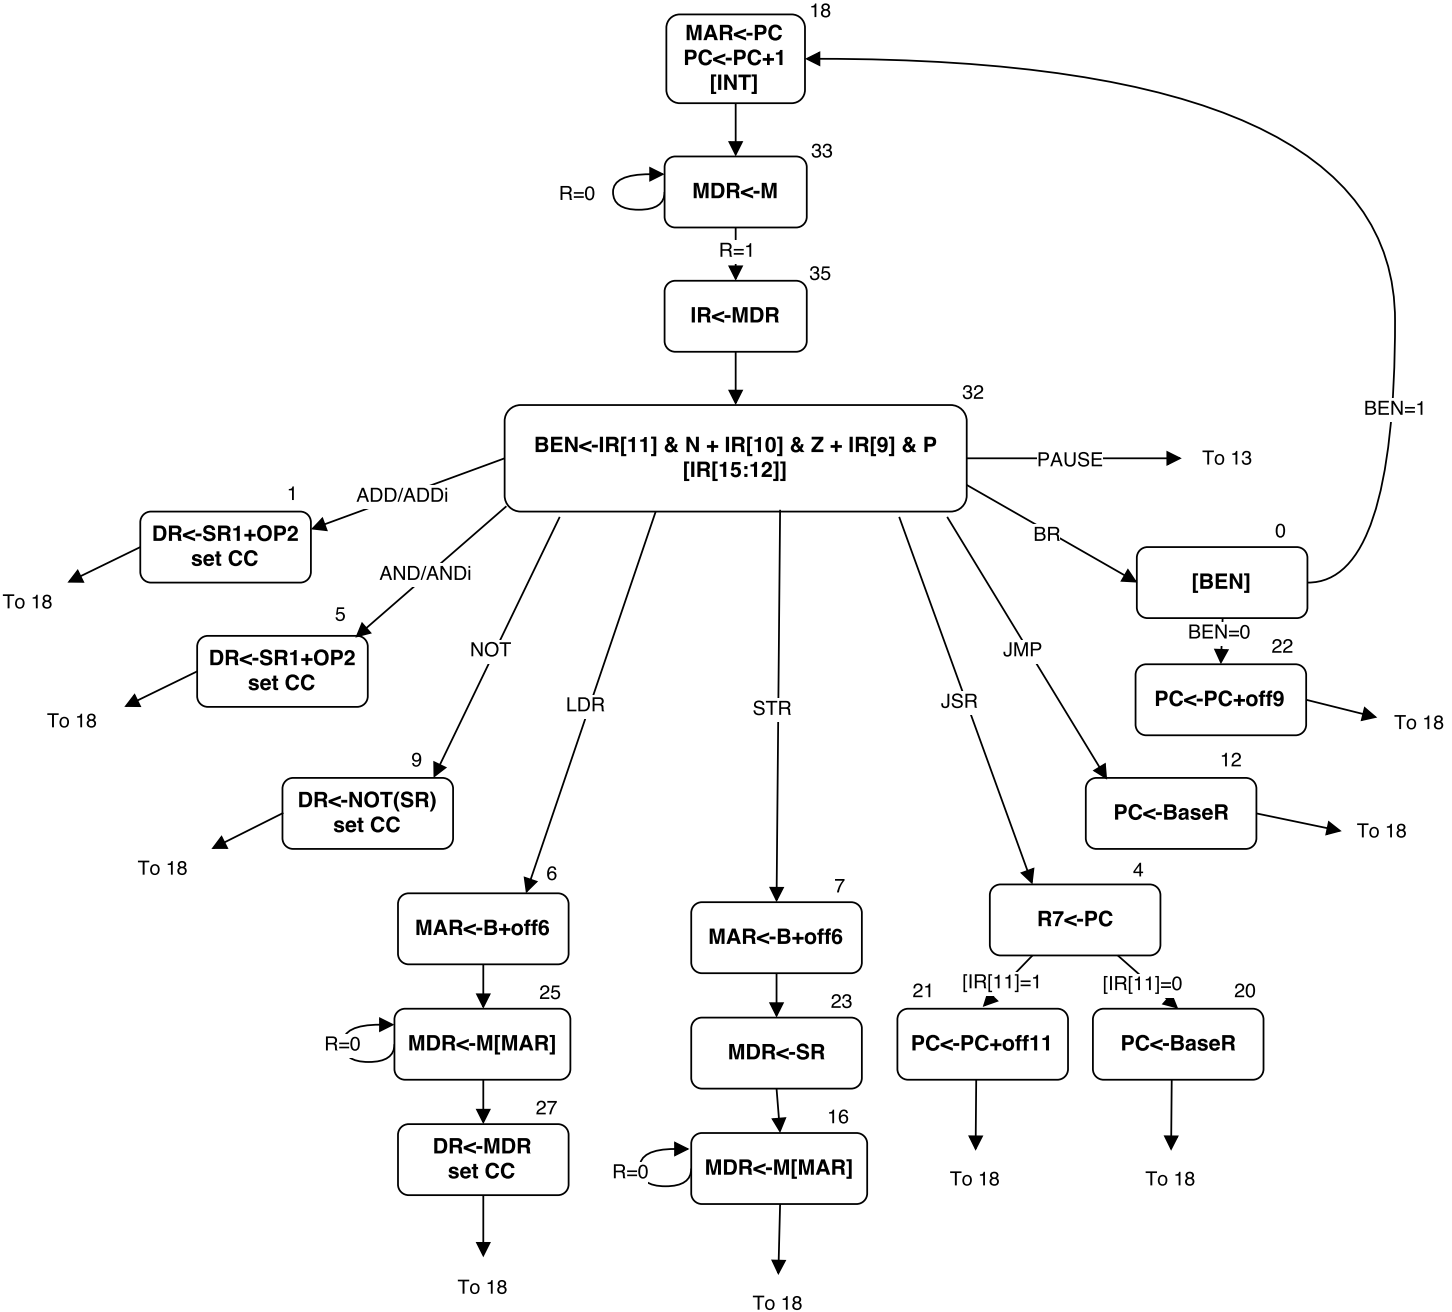
\includegraphics[scale=0.7]{state-diagram.png}
	\caption{SLC3 Machine State Diagram	\label{fig:state-diagram}}
\end{figure}


\begin{figure} [htbp]
	\centering
	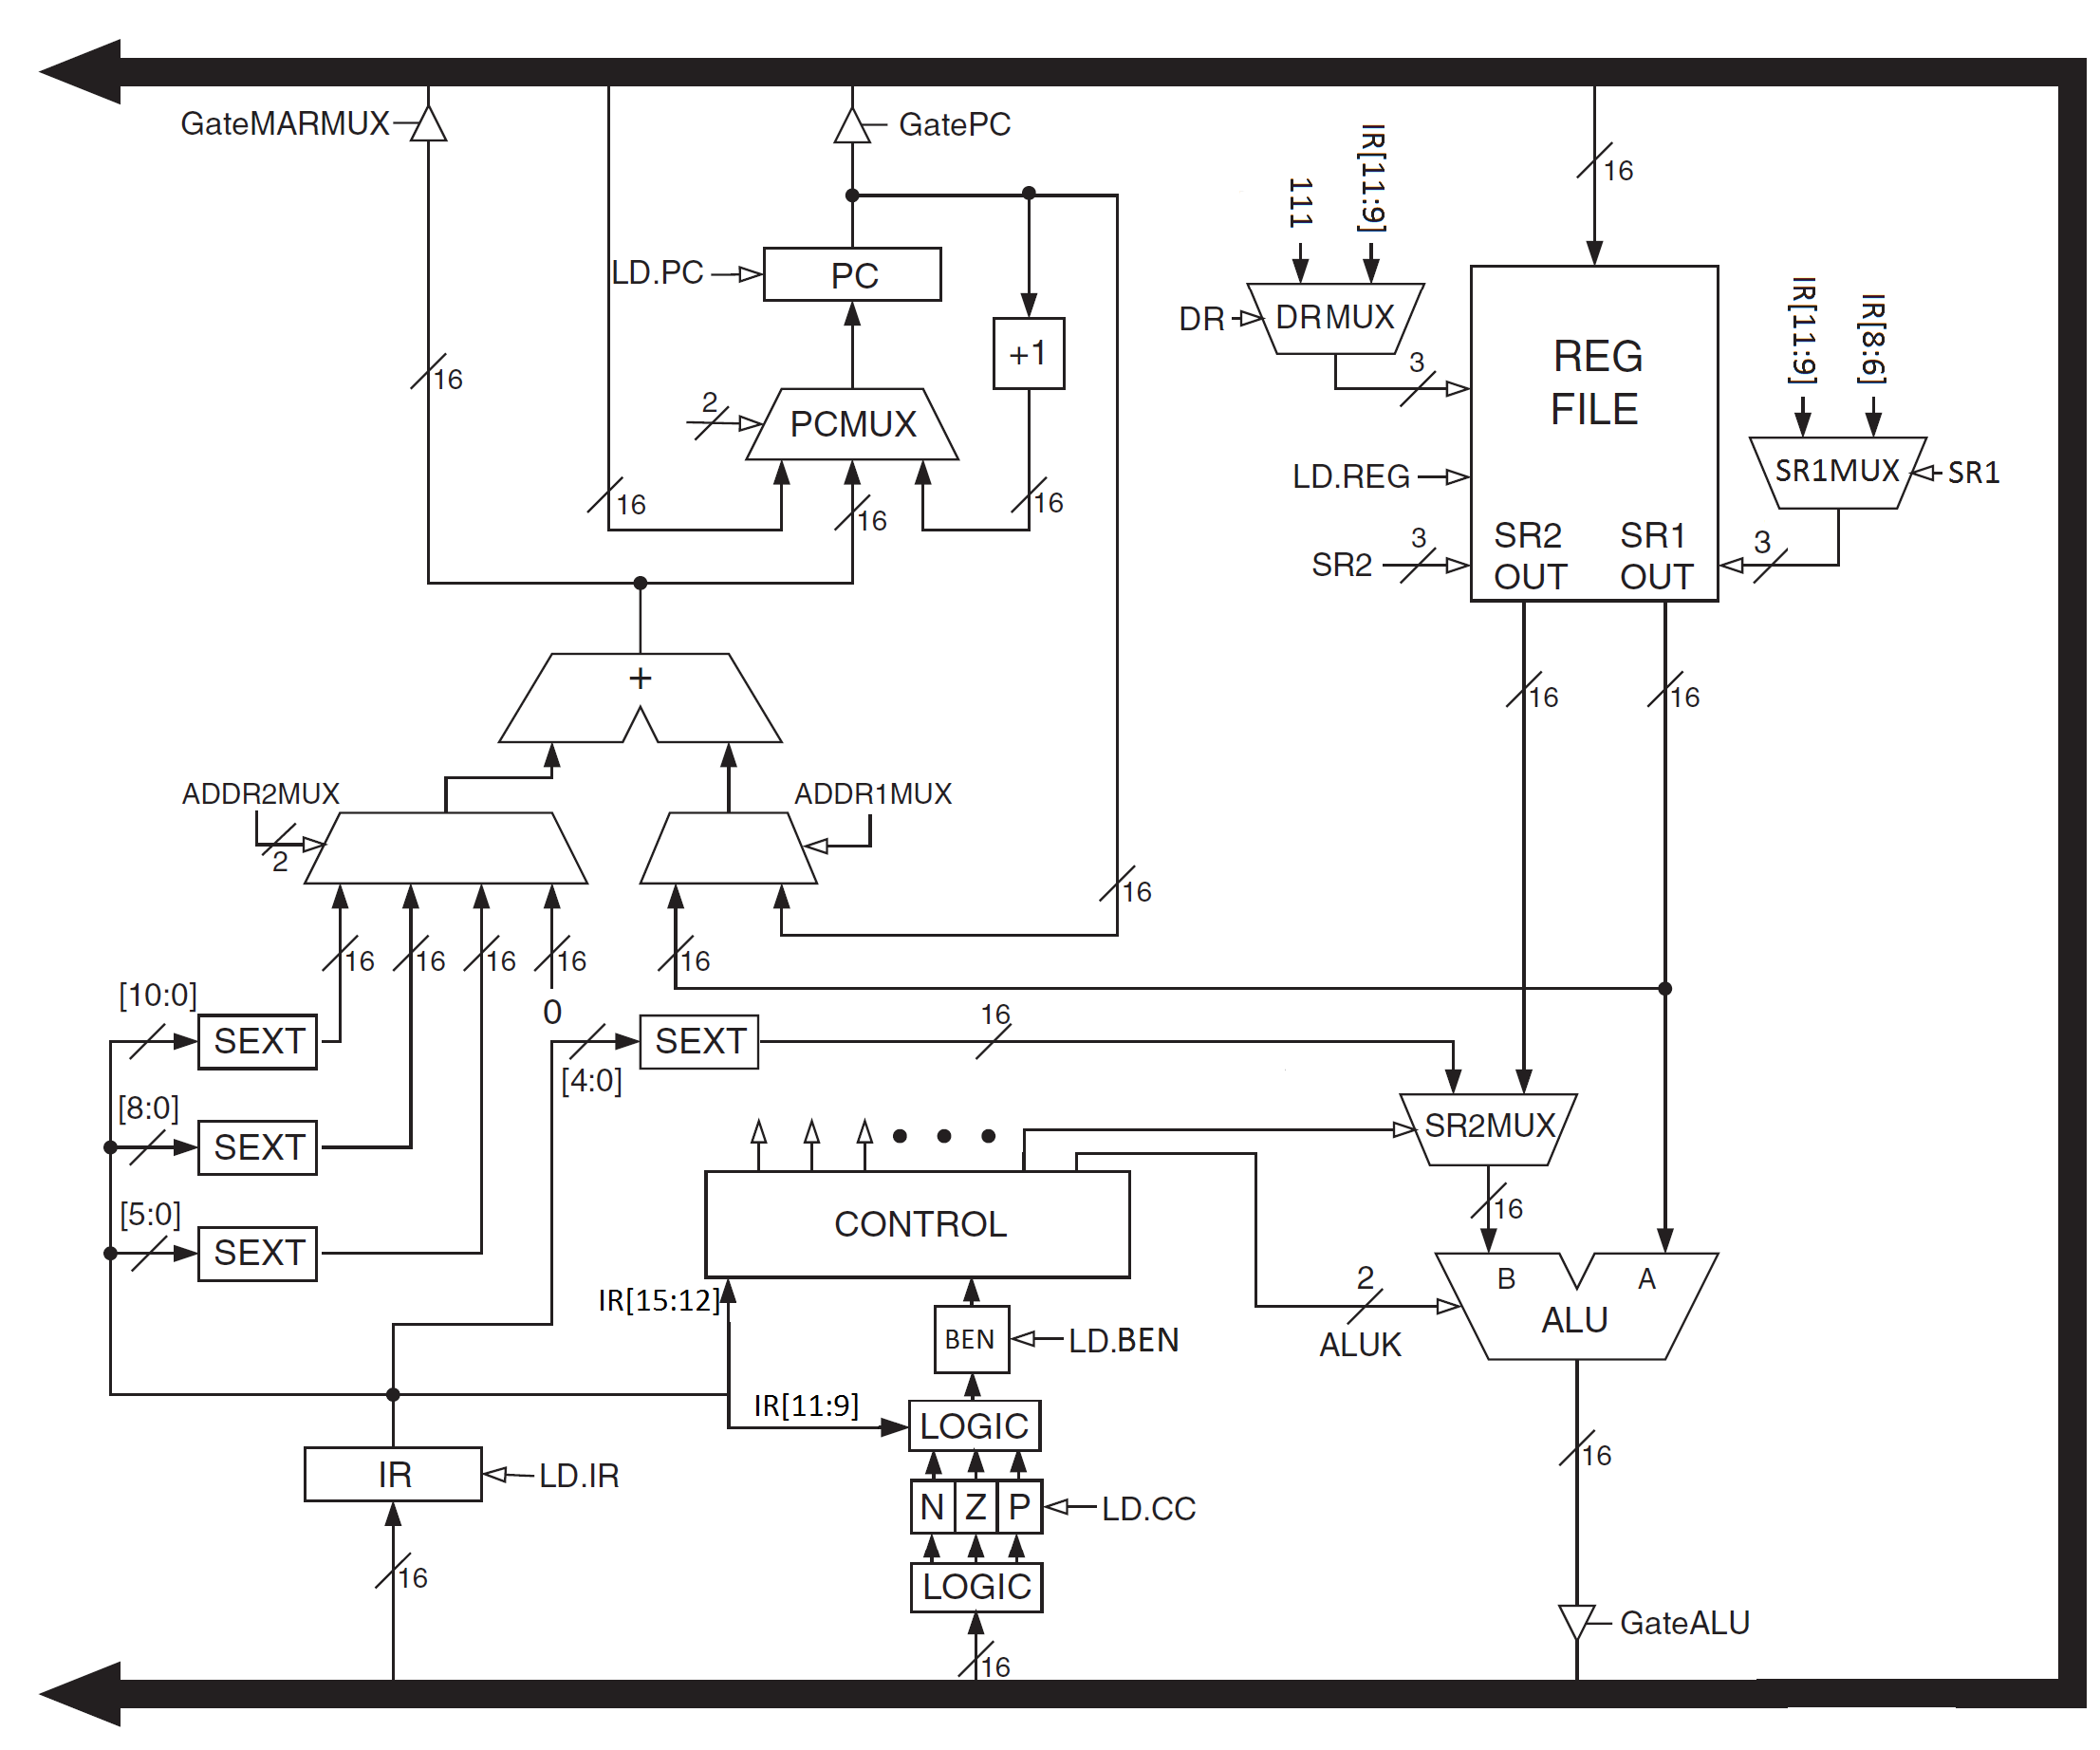
\includegraphics[scale=0.27]{SLC3_Circuit.png}
	\caption{SLC3 CPU \label{fig:SLC3-Circuit}}
\end{figure}

\begin{figure} [htbp]
	\centering
	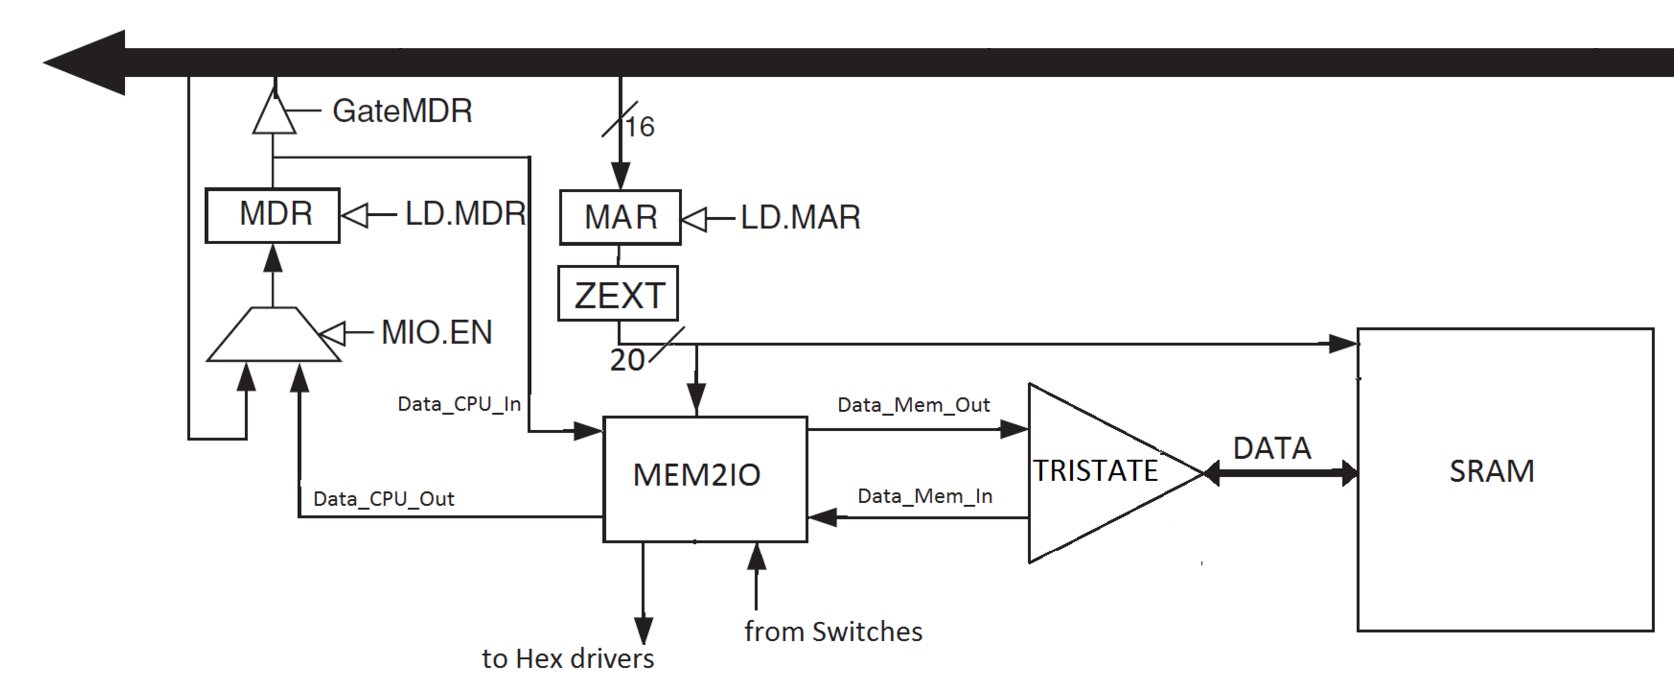
\includegraphics[scale=0.4]{Memory_Circuit.png}
	\caption{Memory, MAR, MDR, Mem2IO Configuration\label{fig:Memory-Circuit}}
\end{figure}

\begin{figure} [htbp]
	\centering
	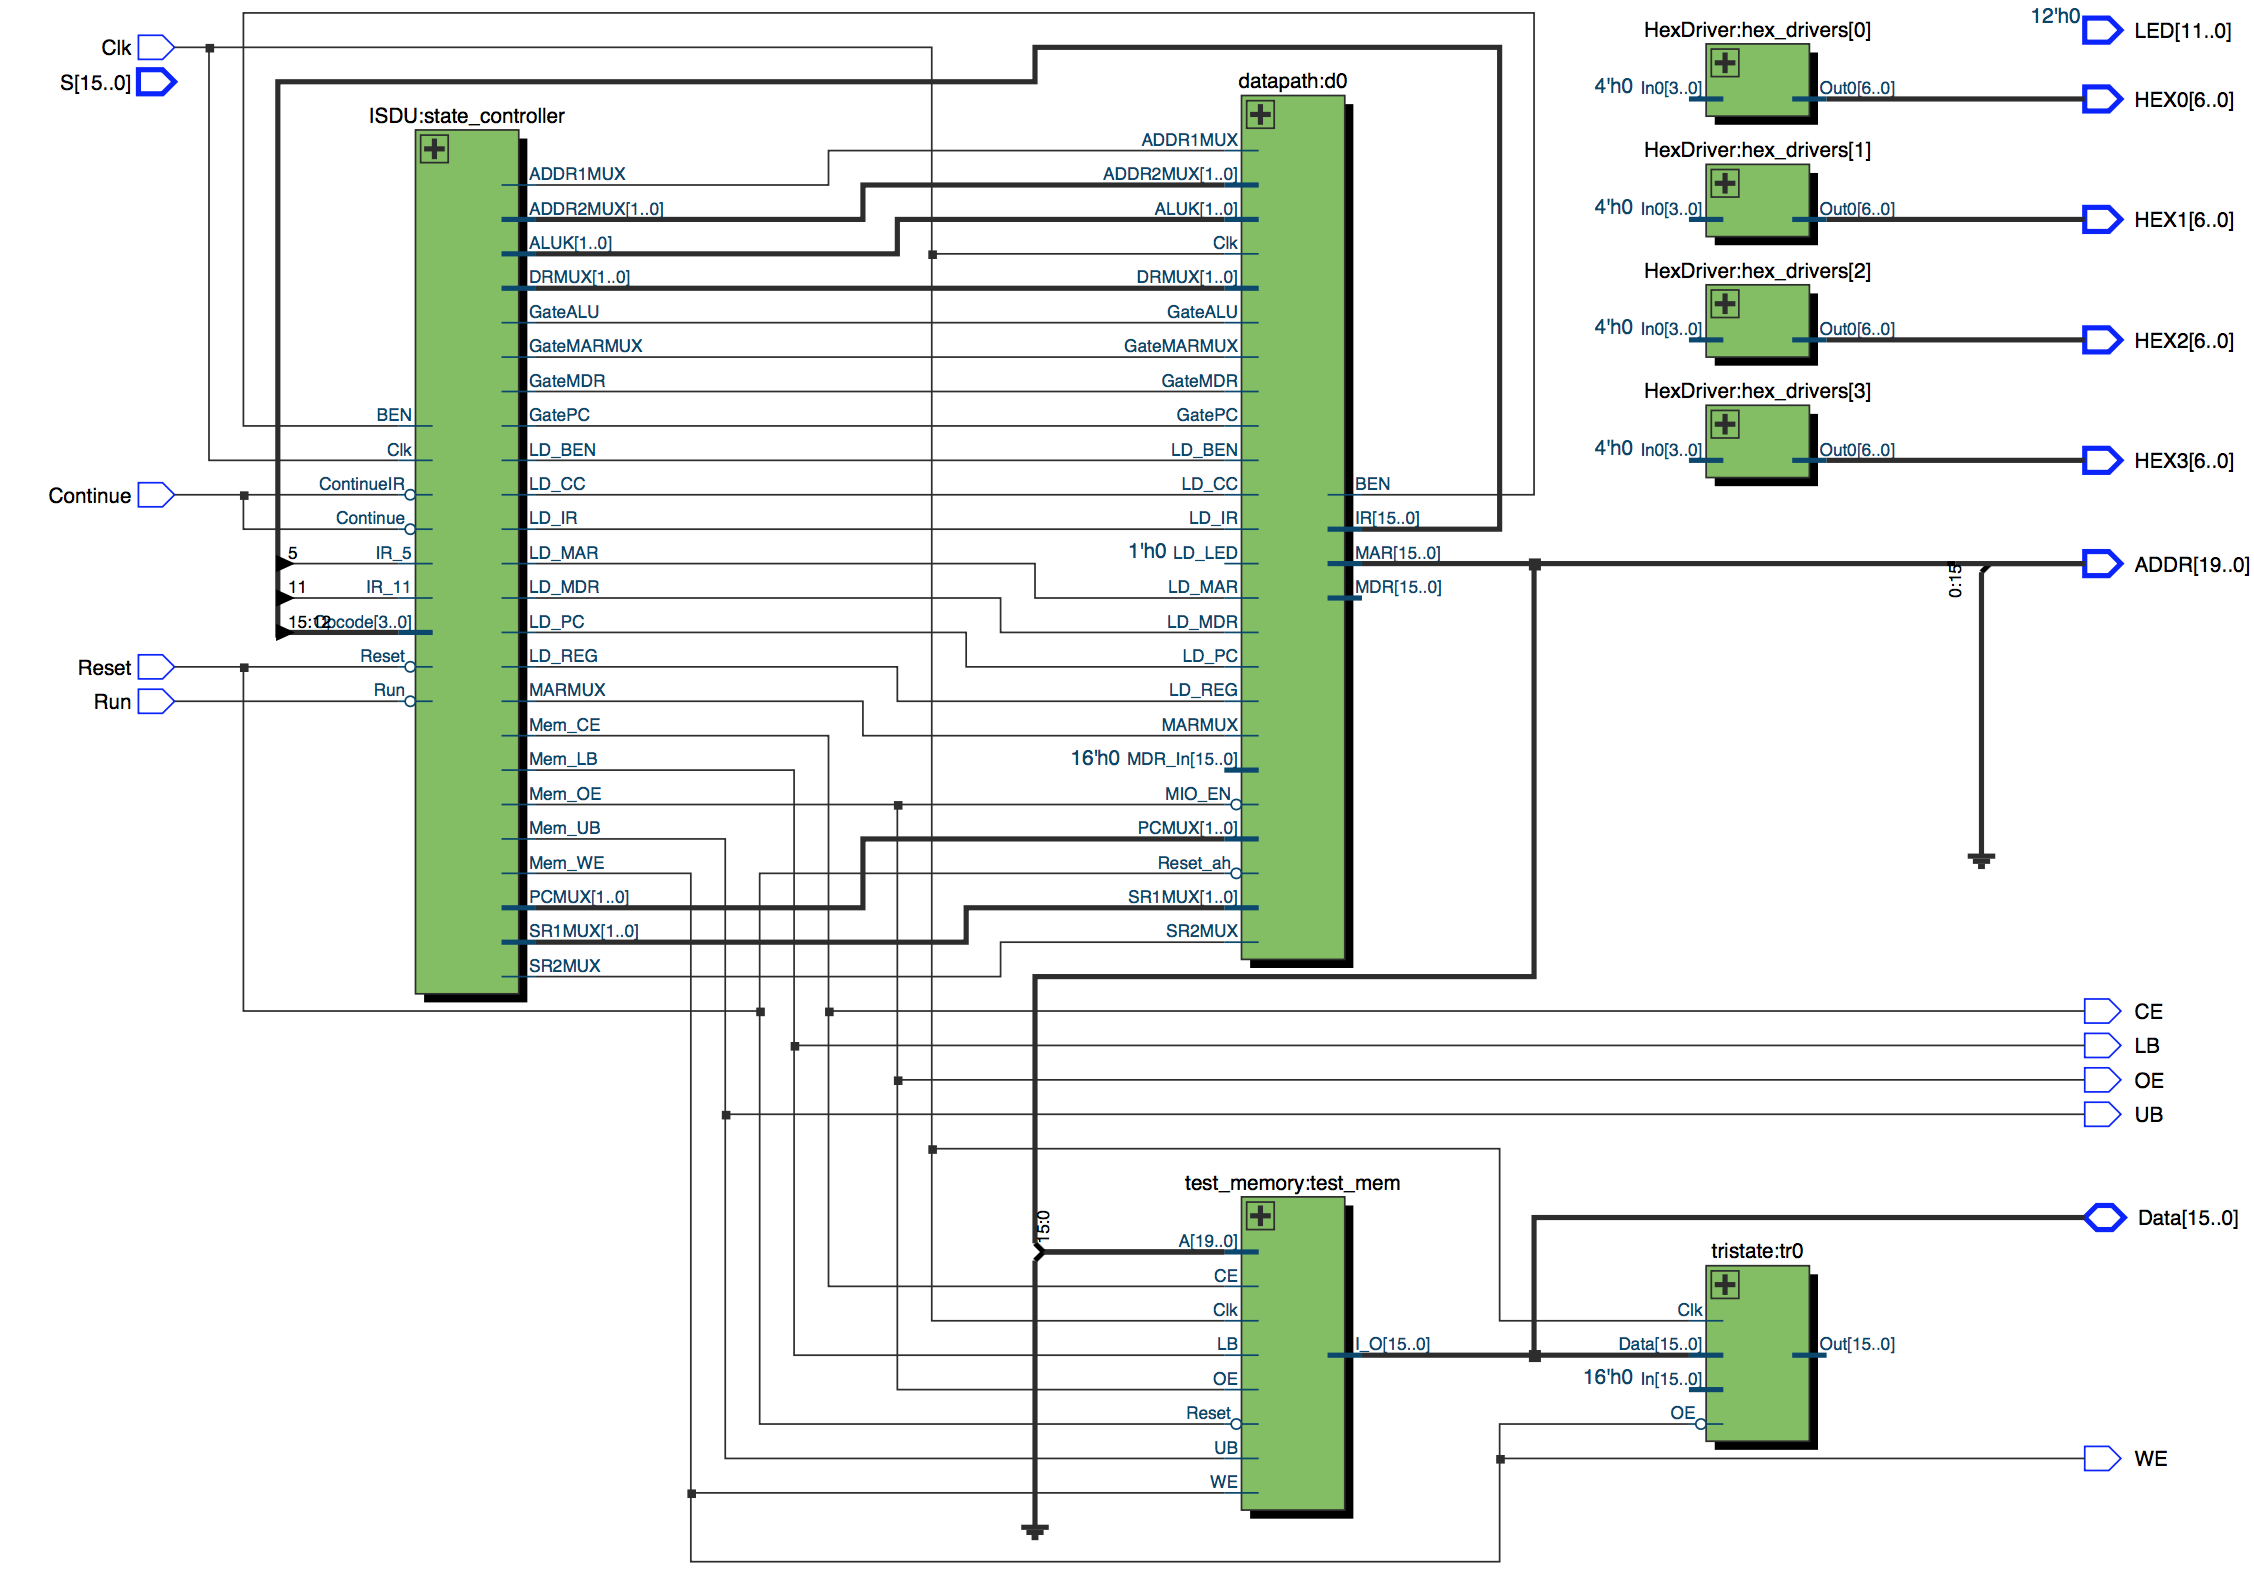
\includegraphics[scale=0.4]{slc3_top_level_circuit.png}
	\caption{SLC3 Top Level Diagram\label{fig:slc3-circuit}}
\end{figure}

\begin{figure} [htbp]
	\centering
	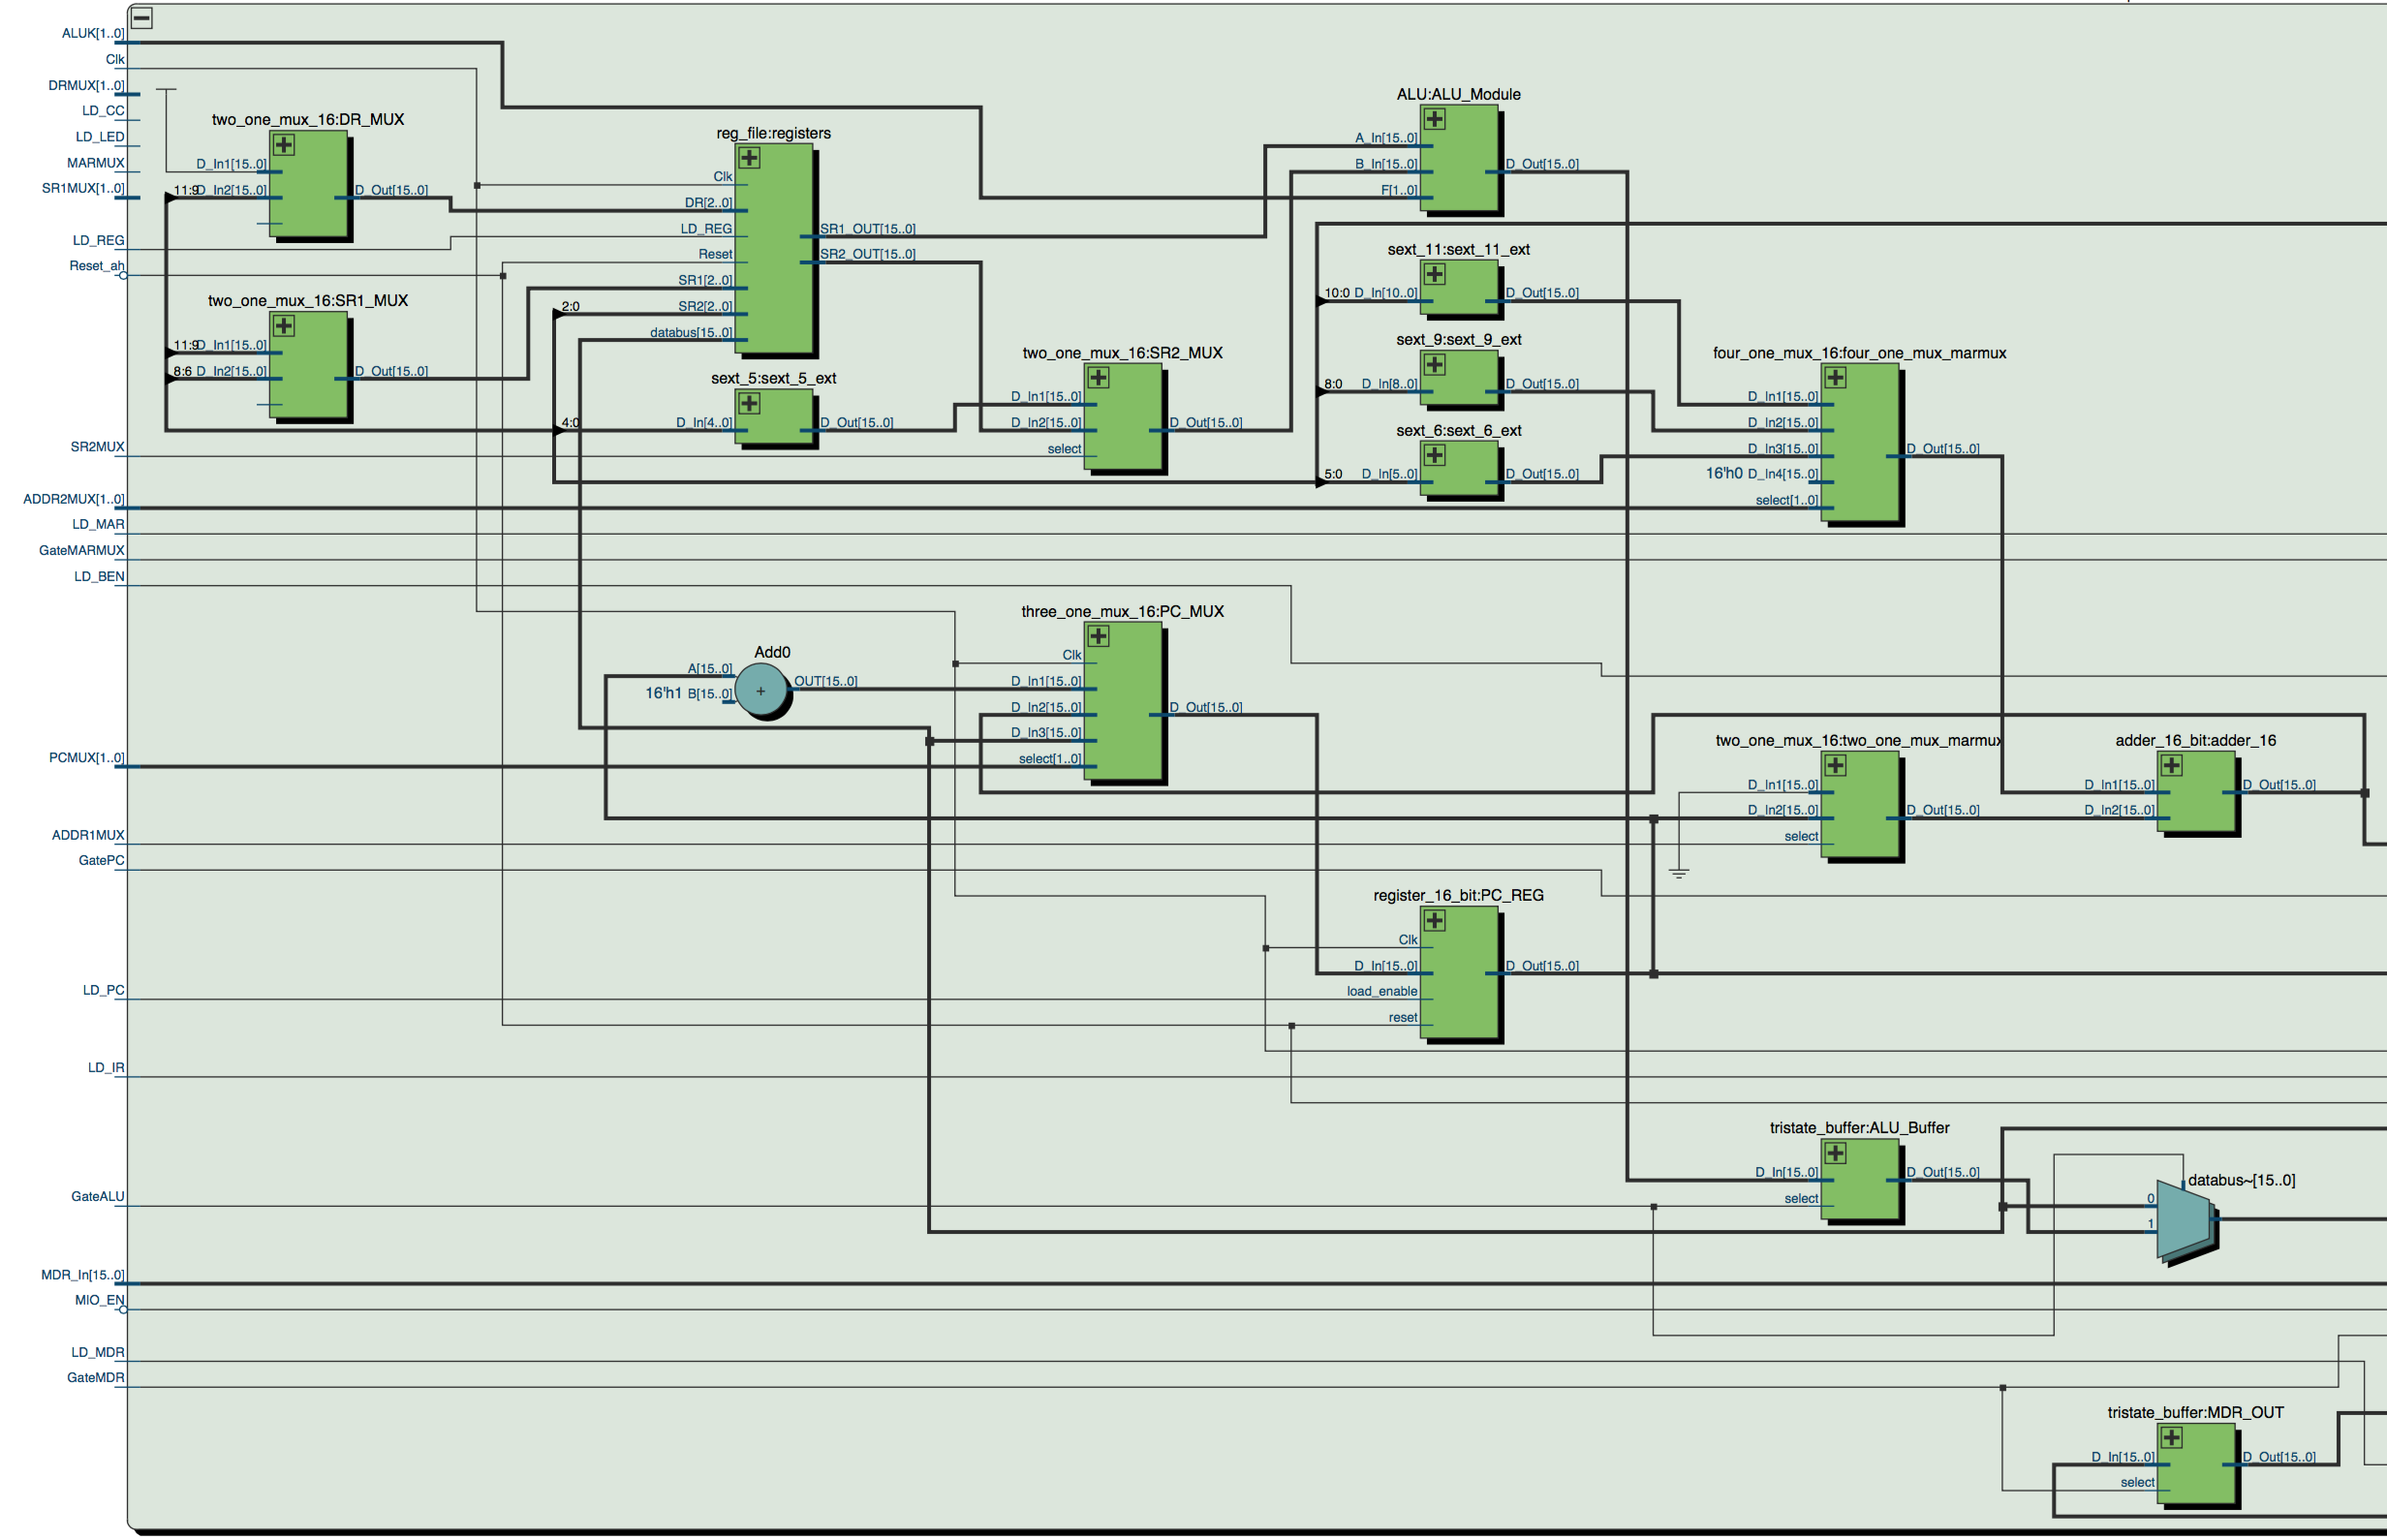
\includegraphics[scale=0.4]{datapath_input_circuit.png}
	\caption{Datapath Circuit Input\label{fig:datapath-circuit-input}}
\end{figure}

\begin{figure} [htbp]
	\centering
	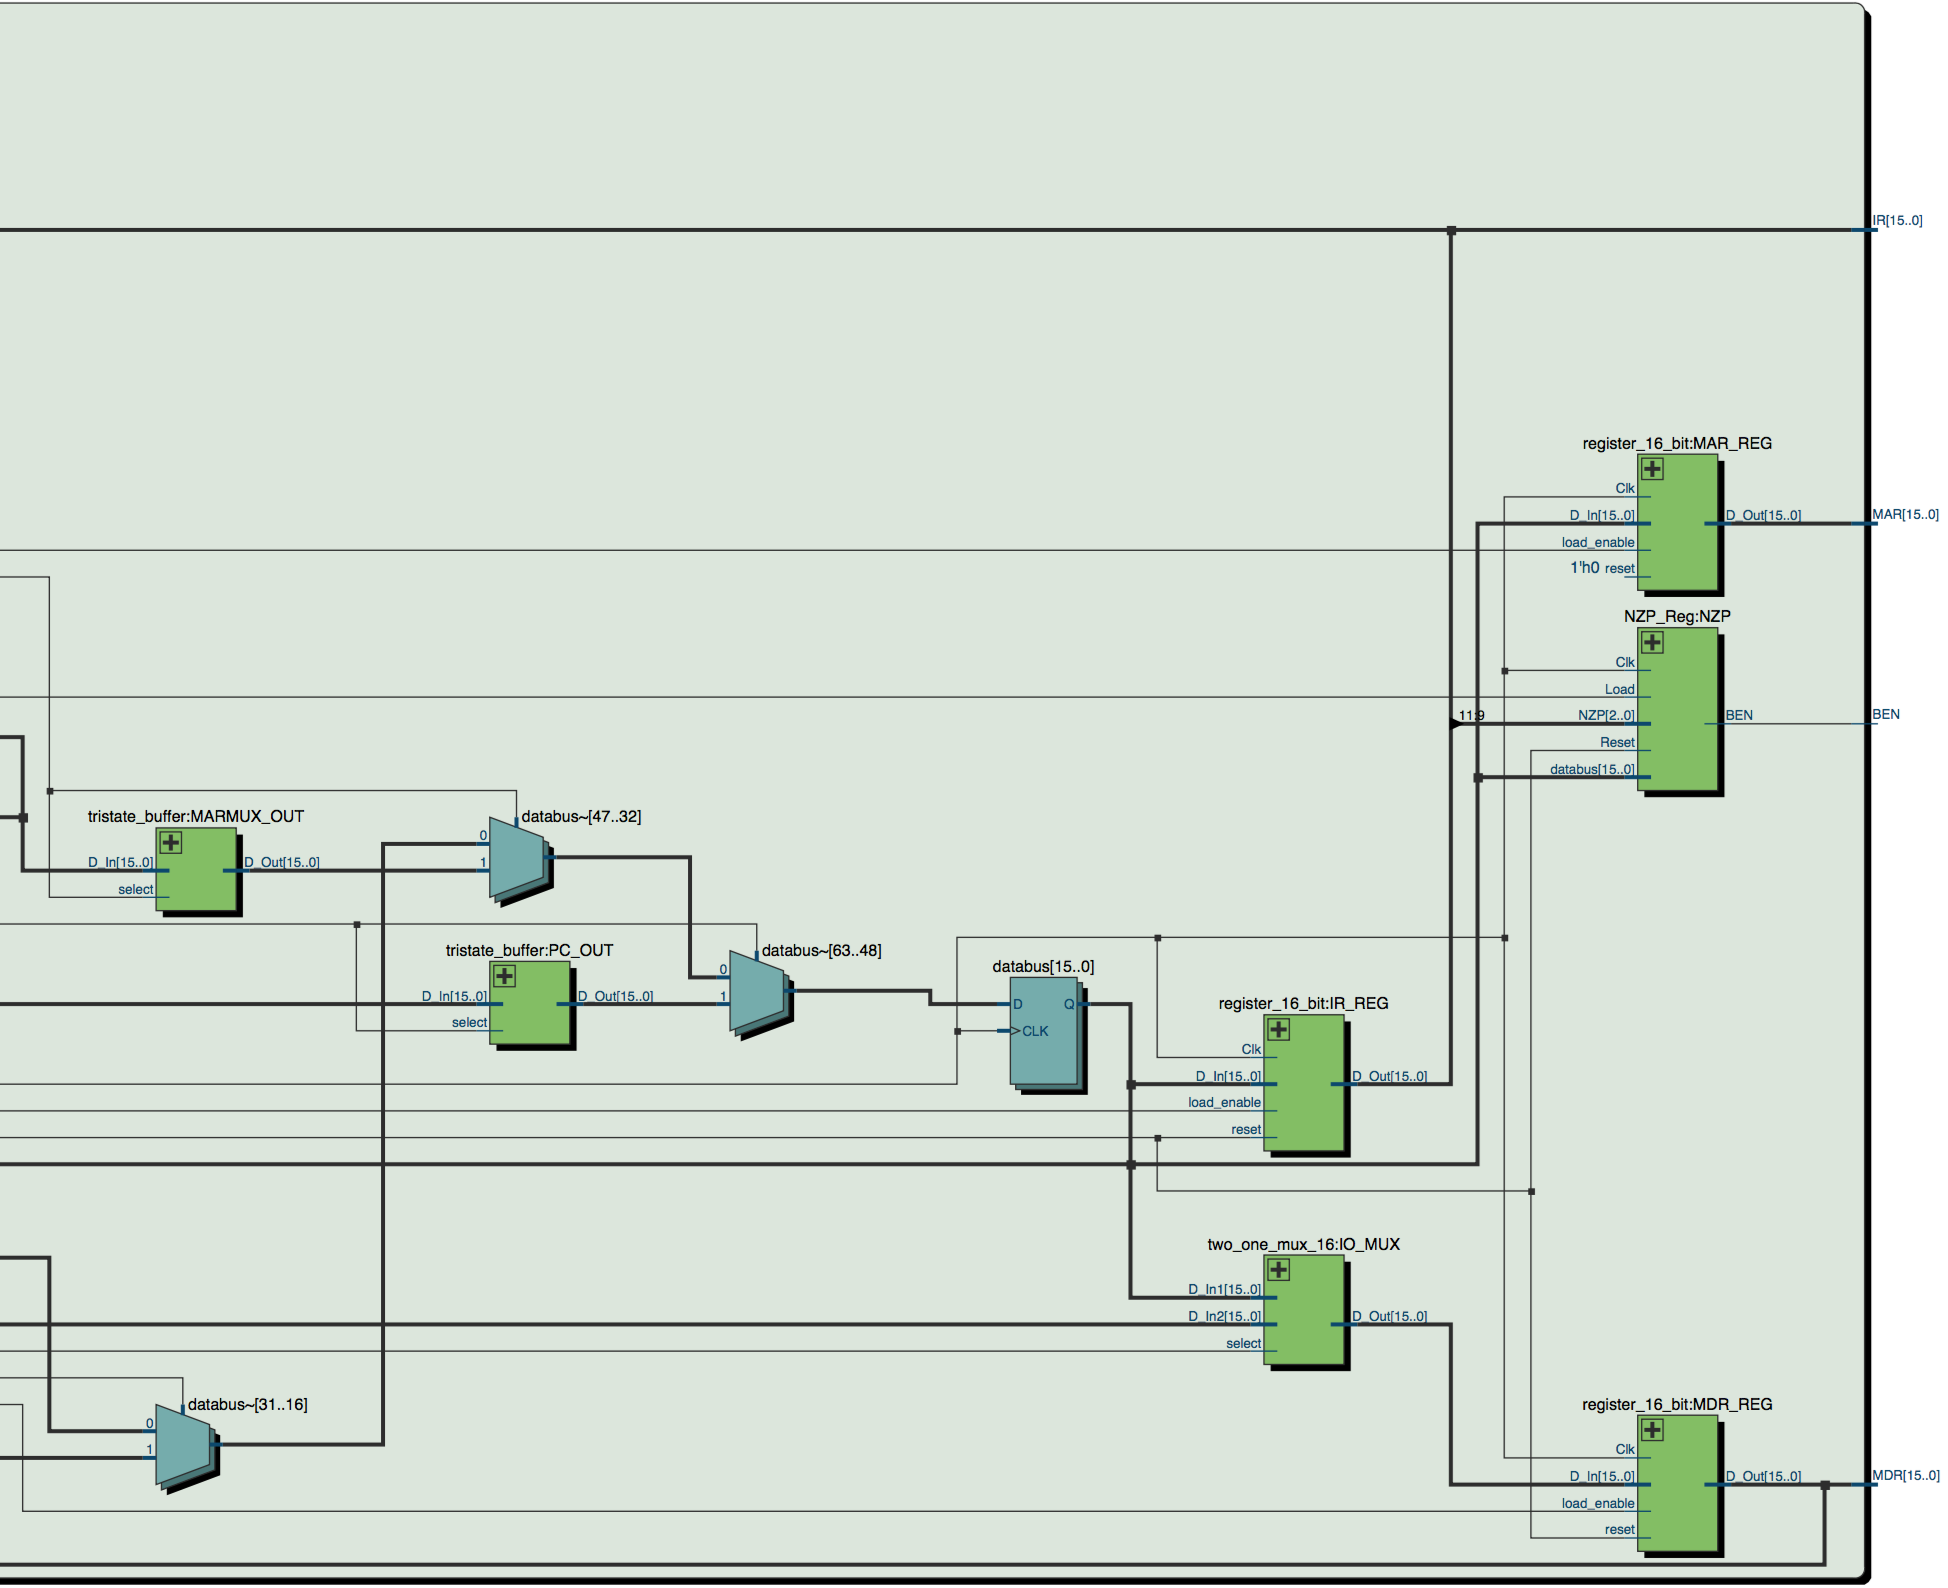
\includegraphics[scale=0.4]{datapath_output_circuit.png}
	\caption{Datapath (Output Only)\label{fig:datapath-circuit-output}}
\end{figure}

\begin{figure} [htbp]
	\centering
	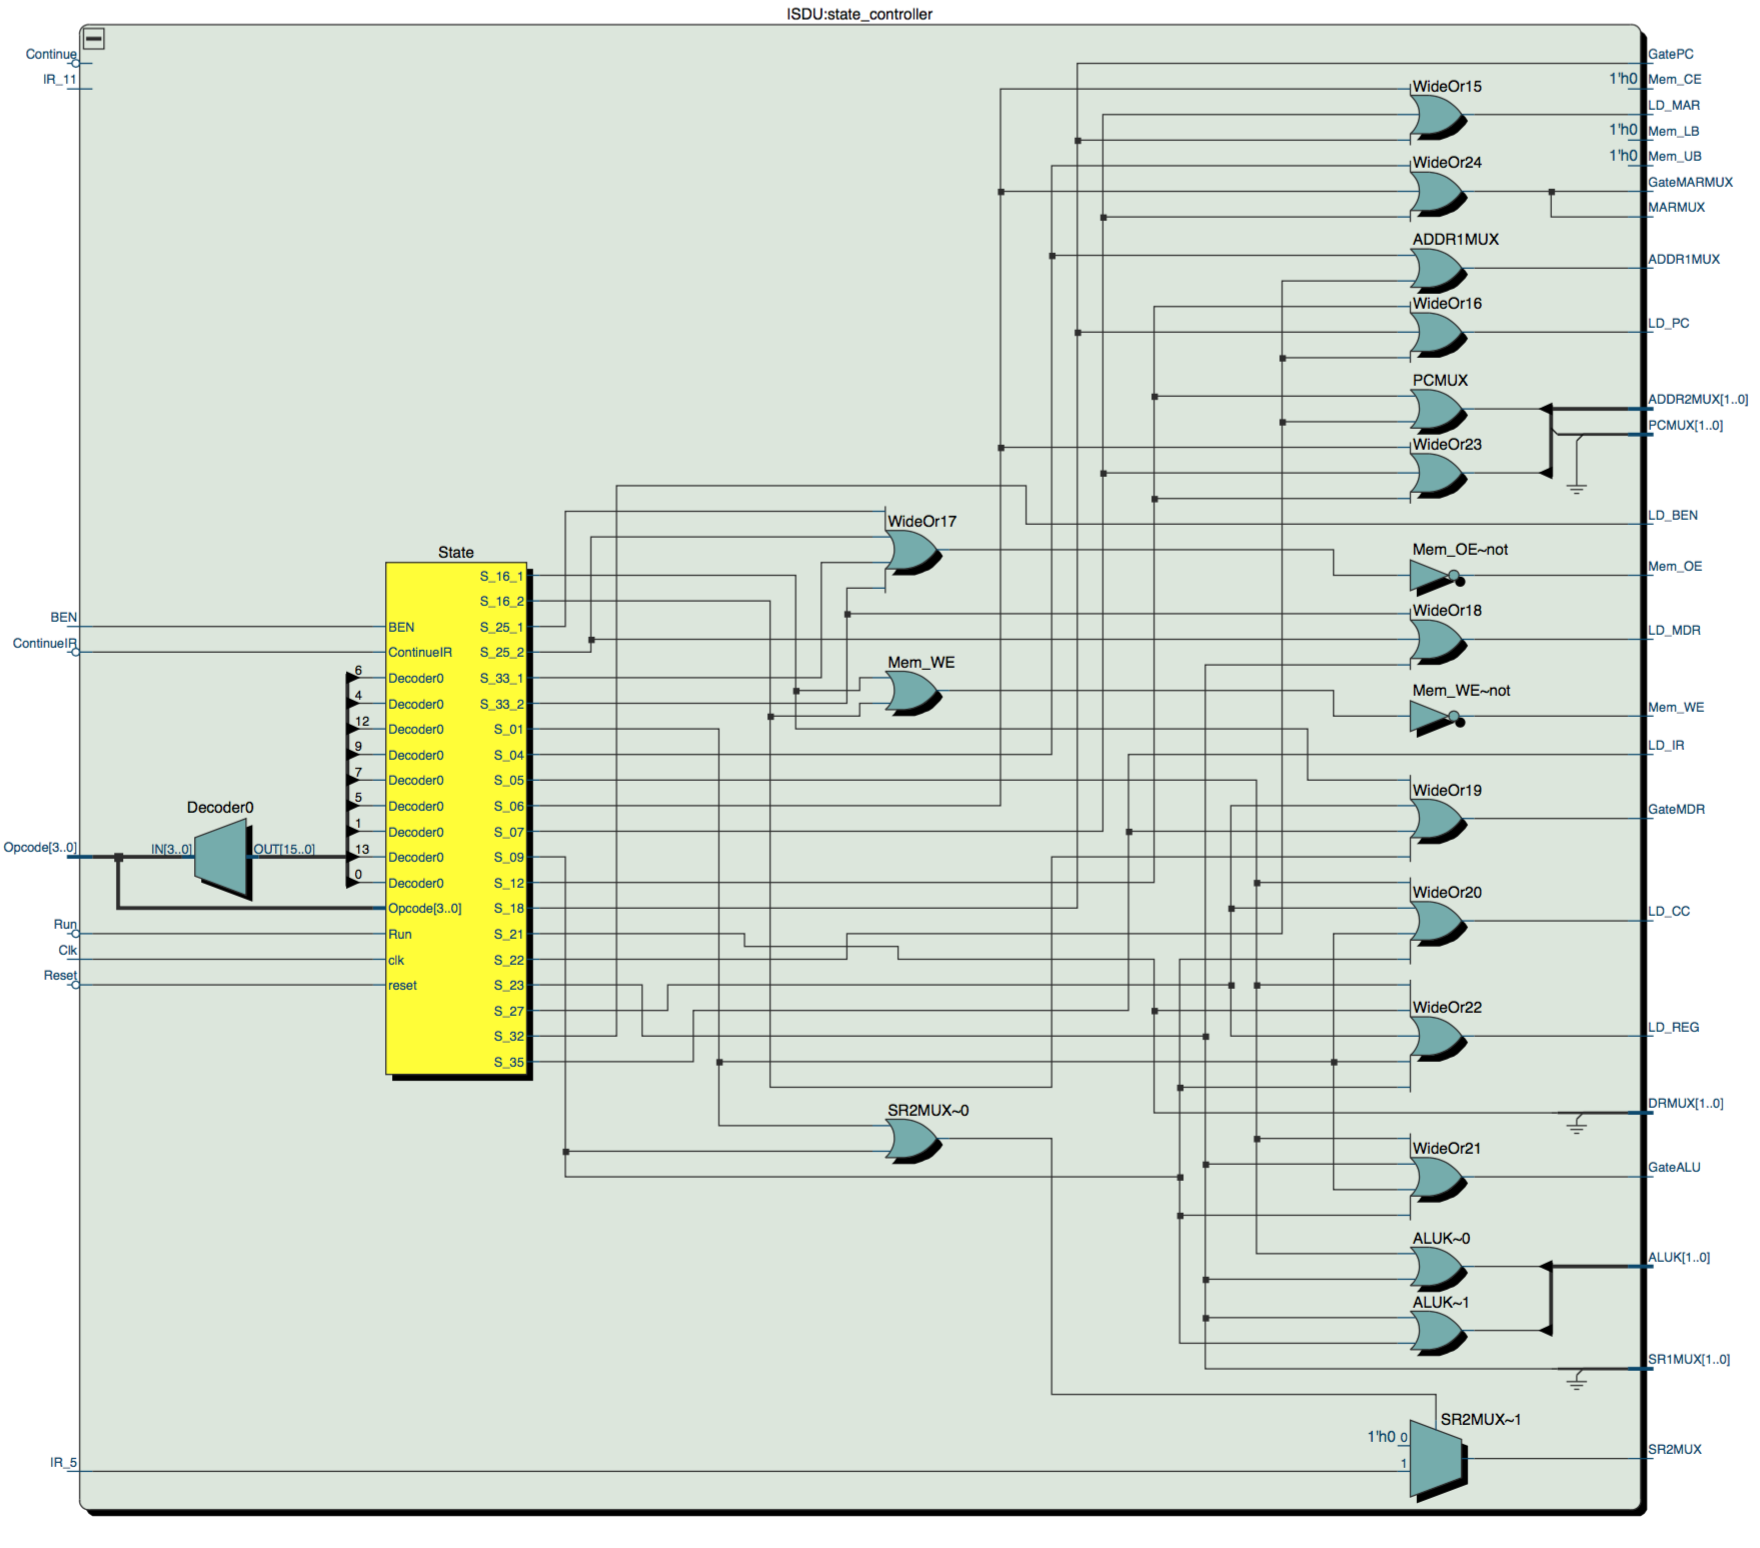
\includegraphics[scale=0.4]{ISDU_Circuit.png}
	\caption{Instruction Sequencer and Decoding Unit Circuit\label{fig:ISDU-circuit}}
\end{figure}

\begin{figure} [htbp]
	\centering
	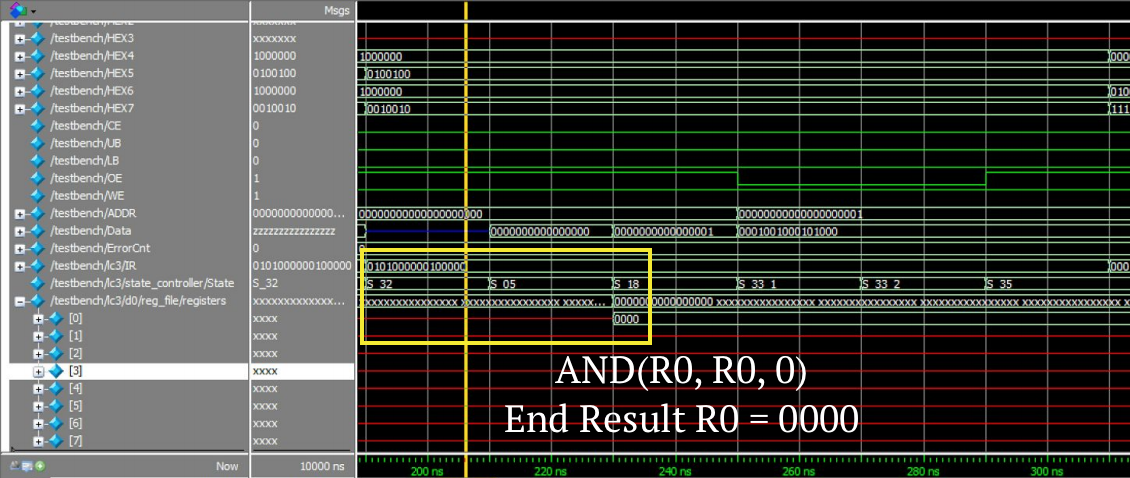
\includegraphics[scale=0.7]{CLR_ANDi.png}
	\caption{Clear and AND Instructions\label{fig:CLR-AND}}
\end{figure}


\begin{figure} [htbp]
	\centering
	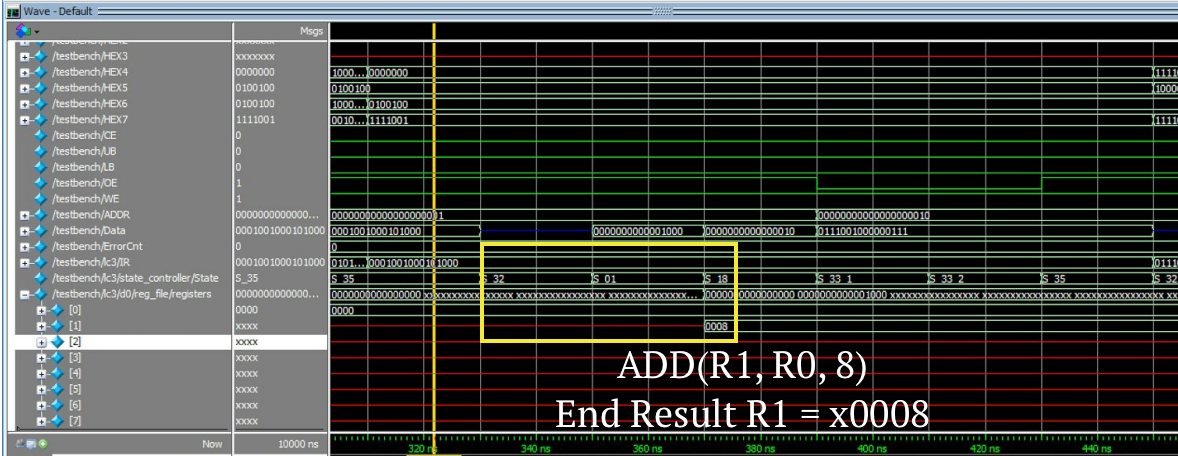
\includegraphics[scale=0.7]{ADDi.png}
	\caption{ADD Immediate Instruction\label{fig:ISDU-circuit}}
\end{figure}


\begin{figure} [htbp]
	\centering
	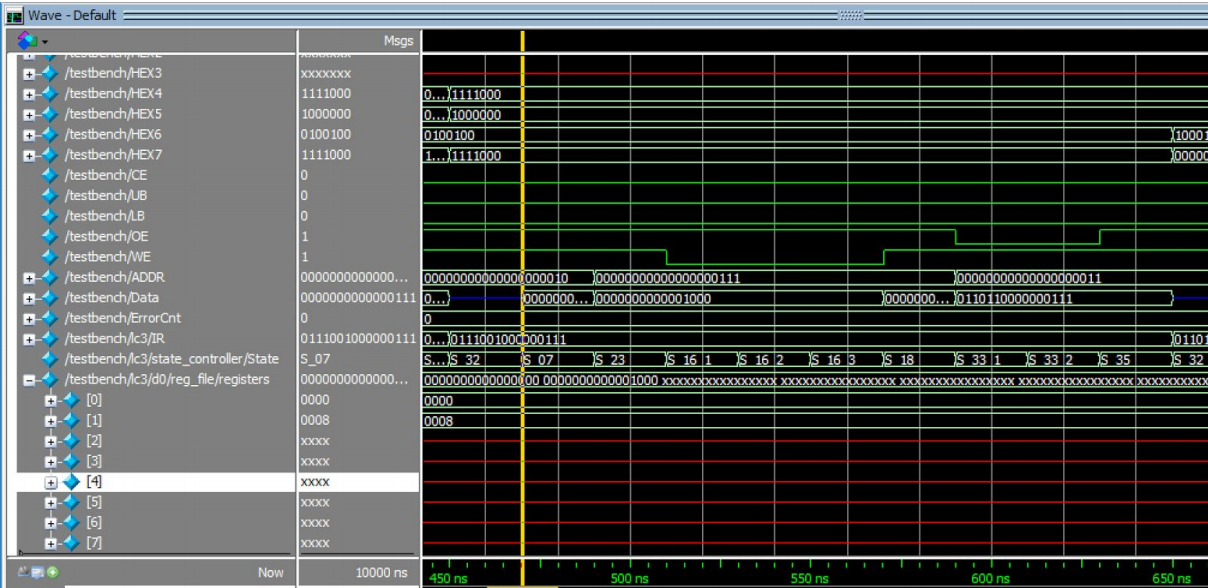
\includegraphics[scale=0.7]{STR.png}
	\caption{Store Register Instructions\label{fig:ISDU-circuit}}
\end{figure}


\begin{figure} [htbp]
	\centering
	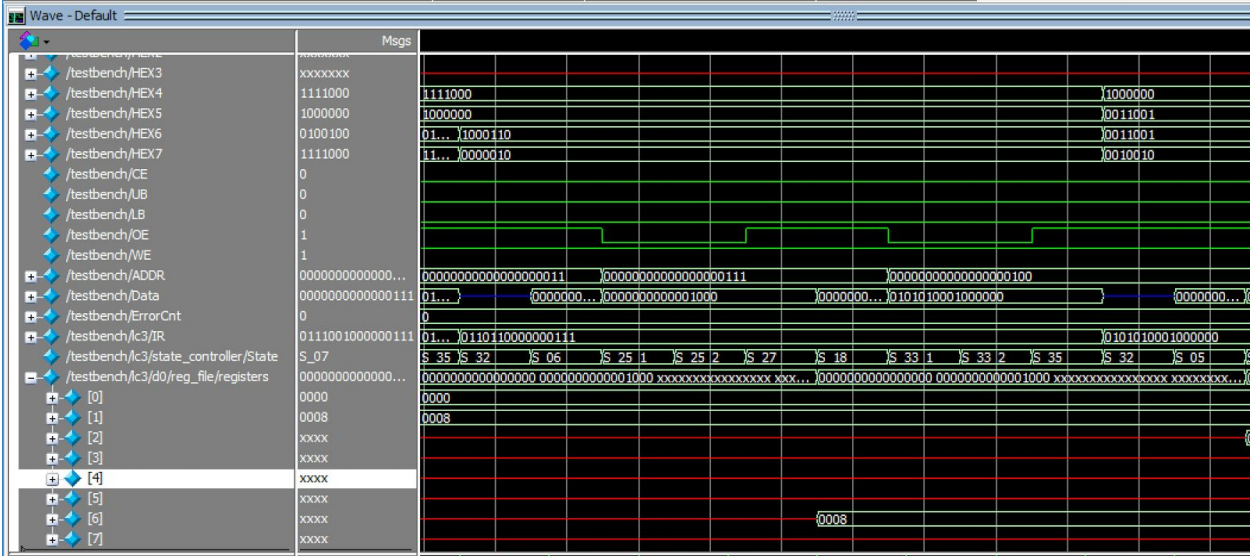
\includegraphics[scale=0.7]{LDR.png}
	\caption{Load Register Instruction\label{fig:ISDU-circuit}}
\end{figure}


\begin{figure} [htbp]
	\centering
	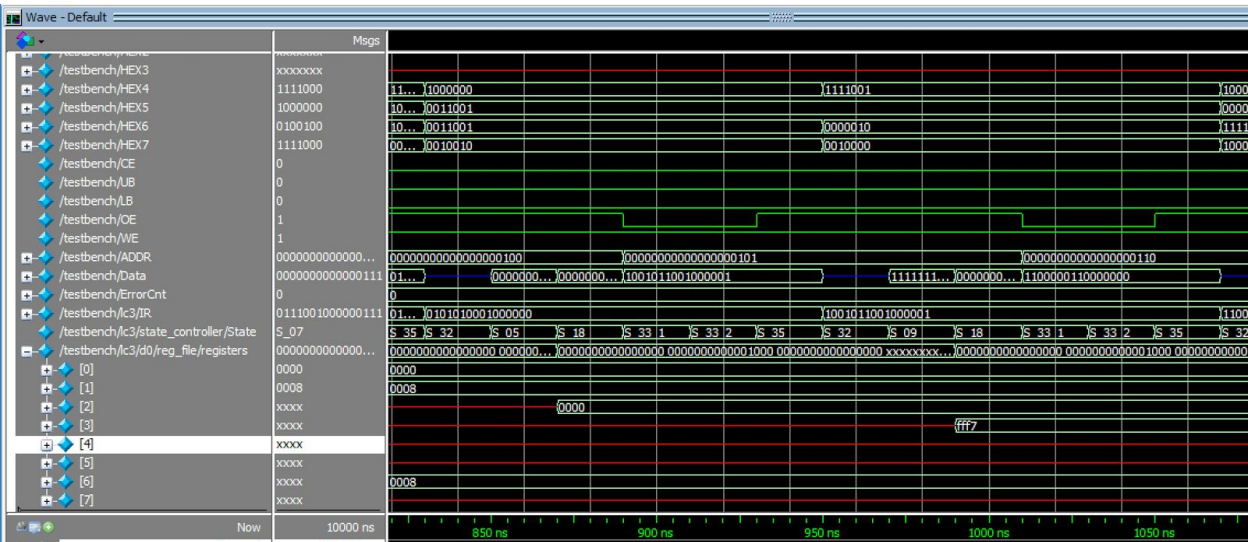
\includegraphics[scale=0.7]{AND_NOT.png}
	\caption{AND and NOT Instructions\label{fig:ISDU-circuit}}
\end{figure}

\begin{figure} [htbp]
	\centering
	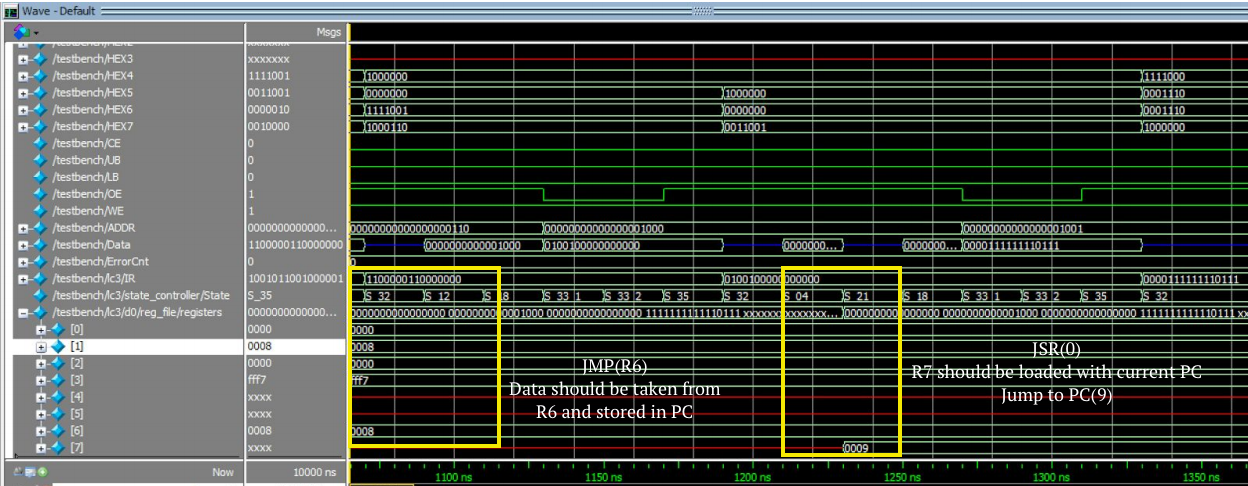
\includegraphics[scale=0.3]{JMP_JSR.png}
	\caption{Jump and Jump Service Routine Instructions\label{fig:ISDU-circuit}}
\end{figure}

\begin{figure} [htbp]
	\centering
	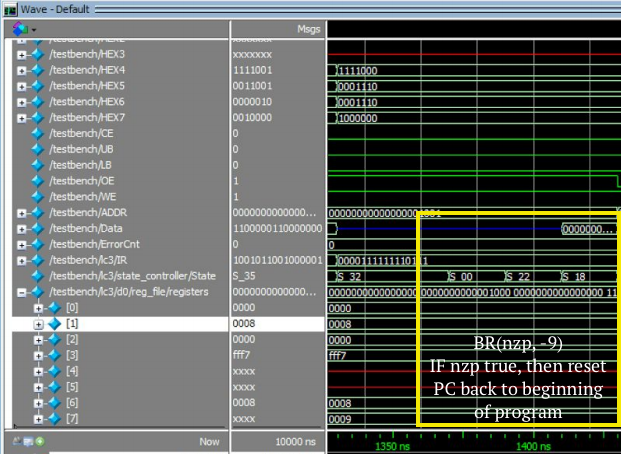
\includegraphics[scale=0.7]{JSR_BR_after.png}
	\caption{Jump and Branch Instructions and End of Testing\label{fig:ISDU-circuit}}
\end{figure}



\clearpage 


\section*{Appendix}
\begin{lstlisting}
always_comb
begin
	case (State)
	Halted: ;
	S_18 : //FETCH - step 1
		begin 
			GatePC = 1'b1;
			LD_MAR = 1'b1;
			PCMUX = 2'b00;
			LD_PC = 1'b1;
		end
	
	S_33_1 : //FETCH - step 2
		begin
			Mem_OE = 1'b0;
		end
	
	S_33_2 : //FETCH - step 3
		begin 
			Mem_OE = 1'b0;
			LD_MDR = 1'b1;
		end
	
	S_35 : //FETCH - step 3
		begin 
			GateMDR = 1'b1;
			LD_IR = 1'b1;
		end
	
	PauseIR1: ;
	
	PauseIR2: ;
	
	S_32 : 
			LD_BEN = 1'b1;
	
	S_01 : //ADD
		begin 
			SR2MUX = IR_5;
			LD_CC = 1'b1;
			ALUK = 2'b00;
			GateALU = 1'b1;
			LD_REG = 1'b1;
		end
	
	S_05:	//AND
		begin
			LD_REG = 1'b1;
			LD_CC = 1'b1;
			ALUK = 2'b10;
			GateALU = 1'b1;
		end
	
	S_09:	//NOT
		begin
			LD_REG = 1'b1;
			LD_CC = 1'b1;
			ALUK = 2'b01;
			GateALU = 1'b1;
			SR2MUX = IR_5;
		end
	
	S_22:	//BR
		begin
			LD_PC = 1'b1;
			PCMUX = 2'b01;
			ADDR1MUX = 1'b1;
			ADDR2MUX = 2'b01;
		end
	
	S_12:	//JMP
		begin
			LD_PC = 1'b1;
			PCMUX = 2'b01;
			ADDR1MUX = 1'b0;
			ADDR2MUX = 2'b11;
		end
	
	S_04:	//JSR - step 1
		begin
			MARMUX = 1'b1;
			GateMARMUX = 1'b1;
			ADDR2MUX = 2'b00;
			ADDR1MUX = 1'b1;
		end
	
	S_21: //JSR - step 2
		begin
			DRMUX = 1'b1;
			LD_REG = 1'b1;
		end
	
	S_06:	//LDR - step 1
		begin
			MARMUX = 1'b1; 
			GateMARMUX = 1'b1;
			ADDR1MUX = 1'b0; 
			ADDR2MUX = 2'b10; 
			LD_MAR = 1'b1;
		end
	
	S_25_1: //LDR - step 2
		begin
			Mem_OE = 1'b0;
		end
	
	S_25_2: //LDR - step 3
		begin
			Mem_OE = 1'b0;
			LD_MDR = 1'b1;
		end
	
	S_27: //LDR - step 4
		begin
			LD_REG = 1'b1;
			LD_CC = 1'b1;
			GateMDR = 1'b1; 
		end
	
	S_07:	//STR - step 1
		begin
			LD_MAR = 1'b1;
			ADDR1MUX = 1'b0; 
			ADDR2MUX = 2'b10; 
			MARMUX = 1'b1; 
			GateMARMUX = 1'b1;
		end
	
	S_23: //STR - step 2
		begin
			SR1MUX = 1'b1; 
			ALUK = 2'b11;
			GateALU = 1'b1;
			LD_MDR = 1'b1;
		end
	
	S_16_1: //STR - step 3
		begin
			Mem_WE = 1'b0; 
			GateMDR = 1'b1; 
		end
	
	S_16_2: //STR - step 4
		begin
			Mem_WE = 1'b0; 
			GateMDR = 1'b1; 
		end
		
	S_16_3: //STR - step 5
		begin
			Mem_WE = 1'b0; 
			GateMDR = 1'b1; 
		end
	
	default : ;
	
	endcase
end
\end{lstlisting}
Test Memory Simulation Setup
\begin{lstlisting}
mem_array[   0 ] <=    opCLR(R0) ;							// Clear R0 can be used as a base
mem_array[   1 ] <=    opADDi(R1, R0, 8) ;				// R1 = R0 + 8
mem_array[   2 ] <=    opSTR(R1, R0, 7) ;				// Store R0 + 7 in R1
mem_array[   3 ] <=    opLDR(R6, R0, 7) ;				// Load R0 + 7 into R6
mem_array[   4 ] <=    opAND(R2, R1, R0) ;				// R2 = R1 & R0
mem_array[   5 ] <=    opNOT(R3, R1) ; 					// R3 = NOT(R1)
mem_array[	 6 ] <=	   opJMP(R6) ; 						// Jump to contents in R6
mem_array[	 7	] <=   opPSE(12'hC02) ;					// WILL NOT REACH THIS STATEMENT
mem_array[   8 ] <=    opJSR(0);							// Jump to 0 (Service Routine)
mem_array[	 9 ] <=    opBR(nzp, -9);					// Branch back to beginning

\end{lstlisting}


%SECTION : Bibliography
%Insert Bibliography if needed

\end{document}
